\chapter{Algoritmi di enumerazione}\label{ch:algoritmi-di-enumerazione}

In informatica, un \textit{algoritmo di enumerazione} \`e un algoritmo che elenca tutte le possibili risposte ad un
problema computazionale in modo sistematico e completo. Tali algoritmi sono quindi progettati per ricevere un
determinato input, generare una lista esaustiva di tutte le possibili soluzioni senza duplicati e, solo allora,
terminare.
Quando si parla di algoritmi di enumerazione applicati al dominio dei grafi, allora spesso si intende il processo di
identificazione di sottoinsiemi di nodi o archi che soddisfano determinate caratteristiche.
In questo capitolo si tratteranno e analizzeranno alcuni utili algoritmi di enumerazione presenti in letteratura per
il riconoscimento di pattern strutturali all'interno di grafi.
In particolare, si discuteranno algoritmi per l'enumerazione di componenti fortemente connesse, di cricche e di
circuiti semplici, problemi di notevole importanza nella teoria dei grafi e ritenuti di interesse per la definizione
di algoritmi di contrazione.
Questi algoritmi costituiranno il \"motore\" degli algoritmi presentati nei capitoli successivi, e saranno di
importanza fondamentale alla definizione degli algoritmi di contrazione usati per la costruzione di grafi multi-livello.

\section{Enumerazione di componenti fortemente connesse}\label{subsec:enumerazione-di-componenti-fortemente-connesse}

Come citato nel Capitolo~\ref{ch:grafi-e-approccio-multi-livello}, la condensazione di un grafo diretto \`e il suo
grafo quoziente dove le componenti fortemente connesse definiscono i blocchi della partizione.
Enumerare le componenti fortemente connesse di un grafo diretto $G = (V, E)$ significa trovare tutti i sottoinsiemi
che permettano di costruire una condensazione del grafo di partenza.
In questa sezione si discuter\`a un classico algoritmo di enumerazione delle componenti fortemente connesse, chiamato
da alcuni testi come l'algoritmo di Kosaraju~\cite{SHARIR198167} e al seguito si discuter\`a di un possibile adattamento
dell'algoritmo per la costruzione contestuale di un grafo contratto in forma di grafo decontraibile.

\subsection{Algoritmo di Kosaraju}\label{subsec:algoritmo-di-kosaraju}

L'algoritmo di Kosaraju (anche noto come algoritmo di Kosaraju-Sharir) è un algoritmo per l'enumerazione
delle componenti fortemente connesse di un grafo diretto dalla complessità lineare scoperto nel 1978 da S. Rao
Kosaraju, ma pubblicato solamente nel 1981 da Micha Sharir, che lo scoprì indipendentemente.
Esso sfrutta il principio per cui le componenti fortemente connesse di un grafo diretto sono le stesse del suo grafo
trasposto, ovvero il grafo ottenuto invertendo l'orientamento di tutti gli archi. \newline

A seguire alcune utili nozioni preliminari per la comprensione dell'algoritmo:

\paragraph{Grafo trasposto}
Dato un grafo diretto $G = (V, E)$, il suo grafo trasposto $G^T = (V, E^T)$ \`e il grafo ottenuto invertendo
l'orientamento di tutti gli archi di $G$, ovvero $E^T = \{(u, v) \mid (v, u) \in E\}$.
 \'E interessante notare che $G^T$ ha le stesse componenti fortemente connesse di $G$: se un cammino da $u$ a $v$
esiste in $G$, allora esiste anche un cammino da $v$ a $u$ in $G^T$.
Essendo le componenti fortemente connesse basate sulla mutua raggiungibilit\`a dei nodi, esse non cambiano
quando si invertono gli archi.

Una procedura algoritmica per il calcolo di $G^T$ non farebbe altro che scorrere linsieme di archi di $G$ e
invertirli, e sarebbe quindi di complessit\`a lineare.

\paragraph{Visita in profondit\`a}
La visita in profondit\`a di un grafo (in inglese \textit{depth-first search} o \textit{DFS}) \`e un particolare
algoritmo di visita che, in quanto tale, permette di visitare tutti i nodi di un grafo partendo da un nodo iniziale,
e di scoprire tutti i nodi raggiungibili da esso.
Ci\`o viene fatto in modo ricorsivo: nel corso della visita di un nodo si considerano uno ad uno i nodi ad esso
adiacenti, e ai nodi non ancora marcati come visitati viene applicata immediatamente la stessa procedura di visita.

\begin{algorithm}[H]
    \caption{DFS($G$)}\label{alg:dfs}
    \begin{algorithmic}[1]
        \For {$v \in G.V$}
            \State $v.color \coloneqq$ WHITE
            \State $u.\pi \coloneqq$ NIL
        \EndFor
        \State $time \coloneqq 0$
        \For{$v \in G.V$}
            \If {$v.color ==$ WHITE}
                \State $DFS-VISIT(G, v)$
            \EndIf
    \end{algorithmic}
\end{algorithm}
\begin{algorithm}
    \caption{DFS-VISIT($G$, $u$)}\label{alg:dfs-visit}
    \begin{algorithmic}[1]
        \State $u.color \coloneqq$ GRAY
        \State $time \coloneqq time + 1$
        \State $u.d \coloneqq time$
        \For {$v \in G.Adj[u]$}
            \If {$v.color ==$ WHITE}
                \State $v.\pi \coloneqq u$
                \State $DFS-VISIT(G, v)$
            \EndIf
        \EndFor
        \State $u.color \coloneqq$ BLACK
        \State $time \coloneqq time + 1$
        \State $u.f \coloneqq time$
    \end{algorithmic}
\end{algorithm}


\begin{figure}
    \resizebox{!}{3.07cm}{
    \begin{tikzpicture}
        %comp 1
        \node[mynode](n1) at (0,0){1};
        \node[mynode](n2) at (1.2,-1){2};
        \node[mynode](n3) at (1.2, 1){4};
        \node[mynode](n4) at (2.4, 0){3};
        \draw[myarrow](n1)--(n2);
        \draw[myarrow](n3)--(n1);
        \draw[myarrow](n4)--(n3);
        \draw[myarrow](n2)--(n4);
        %comp 2
        \node[mynode](n5) at (4,1.2){5};
        \node[mynode](n6) at (4,0){6};
        \node[mynode](n7) at (4, -1.2){7};
        \draw[myarrow](n6) -- (n5);
        \draw[myarrow](n5) to[out=3,in=3] (n7);
        \draw[myarrow](n7) -- (n6);

        %comp edges
        \draw[myarrow](n3) -- (n5);
        \draw[myarrow](n2) -- (n7);
        %comp 3
        \node[mynode](n8) at (6, 2){8};
        %comp 4
        \node[mynode, label=above:{$1$}, fill={rgb:black,1;white,2}](n9) at (8, 2){9};
        \node[mynode](na) at (8.5, 0){10};
        \draw[myarrow](n9) -- (n8);
        \draw[myarrow](na) to[out=3,in=3] (n9);
        \draw[myarrow](n9) -- (na);
        \draw[myarrow](n8) -- (n5);
    \end{tikzpicture} \quad \quad
    \begin{tikzpicture}
        %comp 1
        % \node[mynode, fill=black](n1) at (0,0){\textcolor{white}{1}};
        \node[mynode](n1) at (0,0){1};
        \node[mynode](n2) at (1.2,-1){2};
        \node[mynode](n3) at (1.2, 1){4};
        \node[mynode](n4) at (2.4, 0){3};
        \draw[myarrow](n1)--(n2);
        \draw[myarrow](n3)--(n1);
        \draw[myarrow](n4)--(n3);
        \draw[myarrow](n2)--(n4);
        %comp 2
        \node[mynode](n5) at (4,1.2){5};
        \node[mynode](n6) at (4,0){6};
        \node[mynode](n7) at (4, -1.2){7};
        \draw[myarrow](n6) -- (n5);
        \draw[myarrow](n5) to[out=3,in=3] (n7);
        \draw[myarrow](n7) -- (n6);

        %comp edges
        \draw[myarrow](n3) -- (n5);
        \draw[myarrow](n2) -- (n7);
        %comp 3
        \node[mynode](n8) at (6, 2){8};
        %comp 4
        \node[mynode, label=above:{$1$}, fill={rgb:black,1;white,2}](n9) at (8, 2){9};
        \node[mynode, label=below:{$2$}, fill={rgb:black,1;white,2}](na) at (8.5, 0){10};
        \draw[myarrow](n9) -- (n8);
        \draw[myarrow](na) to[out=3,in=3] (n9);
        \draw[myarrow](n9) -- (na);
        \draw[myarrow](n8) -- (n5);
    \end{tikzpicture}
}
\resizebox{!}{3.07cm}{
    \begin{tikzpicture}
        %comp 1
        \node[mynode](n1) at (0,0){1};
        \node[mynode](n2) at (1.2,-1){2};
        \node[mynode](n3) at (1.2, 1){4};
        \node[mynode](n4) at (2.4, 0){3};
        \draw[myarrow](n1)--(n2);
        \draw[myarrow](n3)--(n1);
        \draw[myarrow](n4)--(n3);
        \draw[myarrow](n2)--(n4);
        %comp 2
        \node[mynode](n5) at (4,1.2){5};
        \node[mynode](n6) at (4,0){6};
        \node[mynode](n7) at (4, -1.2){7};
        \draw[myarrow](n6) -- (n5);
        \draw[myarrow](n5) to[out=3,in=3] (n7);
        \draw[myarrow](n7) -- (n6);

        %comp edges
        \draw[myarrow](n3) -- (n5);
        \draw[myarrow](n2) -- (n7);
        %comp 3
        \node[mynode](n8) at (6, 2){8};
        %comp 4
        \node[mynode, label=above:{$1$}, fill={rgb:black,1;white,2}](n9) at (8, 2){9};
        \node[mynode, label=below:{$2/3$}, fill=black](na) at (8.5, 0){\textcolor{white}{10}};
        \draw[myarrow](n9) -- (n8);
        \draw[myarrow](na) to[out=3,in=3] (n9);
        \draw[myarrow](n9) -- (na);
        \draw[myarrow](n8) -- (n5);
    \end{tikzpicture} \quad \quad
    \begin{tikzpicture}
        %comp 1
        \node[mynode](n1) at (0,0){1};
        \node[mynode](n2) at (1.2,-1){2};
        \node[mynode](n3) at (1.2, 1){4};
        \node[mynode](n4) at (2.4, 0){3};
        \draw[myarrow](n1)--(n2);
        \draw[myarrow](n3)--(n1);
        \draw[myarrow](n4)--(n3);
        \draw[myarrow](n2)--(n4);
        %comp 2
        \node[mynode](n5) at (4,1.2){5};
        \node[mynode](n6) at (4,0){6};
        \node[mynode](n7) at (4, -1.2){7};
        \draw[myarrow](n6) -- (n5);
        \draw[myarrow](n5) to[out=3,in=3] (n7);
        \draw[myarrow](n7) -- (n6);

        %comp edges
        \draw[myarrow](n3) -- (n5);
        \draw[myarrow](n2) -- (n7);
        %comp 3
        \node[mynode, label=above:{$4$}, fill={rgb:black,1;white,2}](n8) at (6, 2){8};
        %comp 4
        \node[mynode, label=above:{$1$}, fill={rgb:black,1;white,2}](n9) at (8, 2){9};
        \node[mynode, label=below:{$2/3$}, fill=black](na) at (8.5, 0){\textcolor{white}{10}};
        \draw[myarrow](n9) -- (n8);
        \draw[myarrow](na) to[out=3,in=3] (n9);
        \draw[myarrow](n9) -- (na);
        \draw[myarrow](n8) -- (n5);
    \end{tikzpicture}
}
\resizebox{!}{3.416cm}{
    \begin{tikzpicture}
        %comp 1

        \node[mynode](n1) at (0,0){1};
        \node[mynode](n2) at (1.2,-1){2};
        \node[mynode](n3) at (1.2, 1){4};
        \node[mynode](n4) at (2.4, 0){3};
        \draw[myarrow](n1)--(n2);
        \draw[myarrow](n3)--(n1);
        \draw[myarrow](n4)--(n3);
        \draw[myarrow](n2)--(n4);
        %comp 2
        \node[mynode, label=above:{$5$}, fill={rgb:black,1;white,2}](n5) at (4,1.2){5};
        \node[mynode](n6) at (4,0){6};
        \node[mynode](n7) at (4, -1.2){7};
        \draw[myarrow](n6) -- (n5);
        \draw[myarrow](n5) to[out=3,in=3] (n7);
        \draw[myarrow](n7) -- (n6);

        %comp edges
        \draw[myarrow](n3) -- (n5);
        \draw[myarrow](n2) -- (n7);
        %comp 3
        \node[mynode, label=above:{$4$}, fill={rgb:black,1;white,2}](n8) at (6, 2){8};
        %comp 4
        \node[mynode, label=above:{$1$}, fill={rgb:black,1;white,2}](n9) at (8, 2){9};
        \node[mynode, label=below:{$2/3$}, fill=black](na) at (8.5, 0){\textcolor{white}{10}};
        \draw[myarrow](n9) -- (n8);
        \draw[myarrow](na) to[out=3,in=3] (n9);
        \draw[myarrow](n9) -- (na);
        \draw[myarrow](n8) -- (n5);
    \end{tikzpicture} \quad \quad
    \begin{tikzpicture}
        %comp 1

        \node[mynode](n1) at (0,0){1};
        \node[mynode](n2) at (1.2,-1){2};
        \node[mynode](n3) at (1.2, 1){4};
        \node[mynode](n4) at (2.4, 0){3};
        \draw[myarrow](n1)--(n2);
        \draw[myarrow](n3)--(n1);
        \draw[myarrow](n4)--(n3);
        \draw[myarrow](n2)--(n4);
        %comp 2
        \node[mynode, label=above:{$5$}, fill={rgb:black,1;white,2}](n5) at (4,1.2){5};
        \node[mynode](n6) at (4,0){6};
        \node[mynode, label=below:{$6$}, fill={rgb:black,1;white,2}](n7) at (4, -1.2){7};
        \draw[myarrow](n6) -- (n5);
        \draw[myarrow](n5) to[out=3,in=3] (n7);
        \draw[myarrow](n7) -- (n6);

        %comp edges
        \draw[myarrow](n3) -- (n5);
        \draw[myarrow](n2) -- (n7);
        %comp 3
        \node[mynode, label=above:{$4$}, fill={rgb:black,1;white,2}](n8) at (6, 2){8};
        %comp 4
        \node[mynode, label=above:{$1$}, fill={rgb:black,1;white,2}](n9) at (8, 2){9};
        \node[mynode, label=below:{$2/3$}, fill=black](na) at (8.5, 0){\textcolor{white}{10}};
        \draw[myarrow](n9) -- (n8);
        \draw[myarrow](na) to[out=3,in=3] (n9);
        \draw[myarrow](n9) -- (na);
        \draw[myarrow](n8) -- (n5);
    \end{tikzpicture}
}
\resizebox{!}{3.416cm}{
    \begin{tikzpicture}
        %comp 1
        \node[mynode](n1) at (0,0){1};
        \node[mynode](n2) at (1.2,-1){2};
        \node[mynode](n3) at (1.2, 1){4};
        \node[mynode](n4) at (2.4, 0){3};
        \draw[myarrow](n1)--(n2);
        \draw[myarrow](n3)--(n1);
        \draw[myarrow](n4)--(n3);
        \draw[myarrow](n2)--(n4);
        %comp 2
        \node[mynode, label=above:{$5$}, fill={rgb:black,1;white,2}](n5) at (4,1.2){5};
        \node[mynode, label=right:{$7$}, fill={rgb:black,1;white,2}](n6) at (4,0){6};
        \node[mynode, label=below:{$6$}, fill={rgb:black,1;white,2}](n7) at (4, -1.2){7};
        \draw[myarrow](n6) -- (n5);
        \draw[myarrow](n5) to[out=3,in=3] (n7);
        \draw[myarrow](n7) -- (n6);

        %comp edges
        \draw[myarrow](n3) -- (n5);
        \draw[myarrow](n2) -- (n7);
        %comp 3
        \node[mynode, label=above:{$4$}, fill={rgb:black,1;white,2}](n8) at (6, 2){8};
        %comp 4
        \node[mynode, label=above:{$1$}, fill={rgb:black,1;white,2}](n9) at (8, 2){9};
        \node[mynode, label=below:{$2/3$}, fill=black](na) at (8.5, 0){\textcolor{white}{10}};
        \draw[myarrow](n9) -- (n8);
        \draw[myarrow](na) to[out=3,in=3] (n9);
        \draw[myarrow](n9) -- (na);
        \draw[myarrow](n8) -- (n5);
    \end{tikzpicture} \quad \quad
    \begin{tikzpicture}
        %comp 1
        \node[mynode](n1) at (0,0){1};
        \node[mynode](n2) at (1.2,-1){2};
        \node[mynode](n3) at (1.2, 1){4};
        \node[mynode](n4) at (2.4, 0){3};
        \draw[myarrow](n1)--(n2);
        \draw[myarrow](n3)--(n1);
        \draw[myarrow](n4)--(n3);
        \draw[myarrow](n2)--(n4);
        %comp 2
        \node[mynode, label=above:{$5$}, fill={rgb:black,1;white,2}](n5) at (4,1.2){5};
        \node[mynode, label=right:{$7/8$}, fill=black](n6) at (4,0){\textcolor{white}{6}};
        \node[mynode, label=below:{$6$}, fill={rgb:black,1;white,2}](n7) at (4, -1.2){7};
        \draw[myarrow](n6) -- (n5);
        \draw[myarrow](n5) to[out=3,in=3] (n7);
        \draw[myarrow](n7) -- (n6);

        %comp edges
        \draw[myarrow](n3) -- (n5);
        \draw[myarrow](n2) -- (n7);
        %comp 3
        \node[mynode, label=above:{$4$}, fill={rgb:black,1;white,2}](n8) at (6, 2){8};
        %comp 4
        \node[mynode, label=above:{$1$}, fill={rgb:black,1;white,2}](n9) at (8, 2){9};
        \node[mynode, label=below:{$2/3$}, fill=black](na) at (8.5, 0){\textcolor{white}{10}};
        \draw[myarrow](n9) -- (n8);
        \draw[myarrow](na) to[out=3,in=3] (n9);
        \draw[myarrow](n9) -- (na);
        \draw[myarrow](n8) -- (n5);
    \end{tikzpicture}
}
\resizebox{!}{3.5cm}{
    \begin{tikzpicture}
        %comp 1
        \node[mynode](n1) at (0,0){1};
        \node[mynode](n2) at (1.2,-1){2};
        \node[mynode](n3) at (1.2, 1){4};
        \node[mynode](n4) at (2.4, 0){3};
        \draw[myarrow](n1)--(n2);
        \draw[myarrow](n3)--(n1);
        \draw[myarrow](n4)--(n3);
        \draw[myarrow](n2)--(n4);
        %comp 2
        \node[mynode, label=above:{$5$}, fill={rgb:black,1;white,2}](n5) at (4,1.2){5};
        \node[mynode, label=right:{$7/8$}, fill=black](n6) at (4,0){\textcolor{white}{6}};
        \node[mynode, label=below:{$6/9$}, fill=black](n7) at (4, -1.2){\textcolor{white}{7}};
        \draw[myarrow](n6) -- (n5);
        \draw[myarrow](n5) to[out=3,in=3] (n7);
        \draw[myarrow](n7) -- (n6);

        %comp edges
        \draw[myarrow](n3) -- (n5);
        \draw[myarrow](n2) -- (n7);
        %comp 3
        \node[mynode, label=above:{$4$}, fill={rgb:black,1;white,2}](n8) at (6, 2){8};
        %comp 4
        \node[mynode, label=above:{$1$}, fill={rgb:black,1;white,2}](n9) at (8, 2){9};
        \node[mynode, label=below:{$2/3$}, fill=black](na) at (8.5, 0){\textcolor{white}{10}};
        \draw[myarrow](n9) -- (n8);
        \draw[myarrow](na) to[out=3,in=3] (n9);
        \draw[myarrow](n9) -- (na);
        \draw[myarrow](n8) -- (n5);
    \end{tikzpicture} \quad \quad
    \begin{tikzpicture}
        % comp 1
        \node[mynode](n1) at (0,0){1};
        \node[mynode](n2) at (1.2,-1){2};
        \node[mynode](n3) at (1.2, 1){4};
        \node[mynode](n4) at (2.4, 0){3};
        \draw[myarrow](n1)--(n2);
        \draw[myarrow](n3)--(n1);
        \draw[myarrow](n4)--(n3);
        \draw[myarrow](n2)--(n4);
        %comp 2
        \node[mynode, label=above:{$5/10$}, fill=black](n5) at (4,1.2){\textcolor{white}{5}};
        \node[mynode, label=right:{$7/8$}, fill=black](n6) at (4,0){\textcolor{white}{6}};
        \node[mynode, label=below:{$6/9$}, fill=black](n7) at (4, -1.2){\textcolor{white}{7}};
        \draw[myarrow](n6) -- (n5);
        \draw[myarrow](n5) to[out=3,in=3] (n7);
        \draw[myarrow](n7) -- (n6);

        %comp edges
        \draw[myarrow](n3) -- (n5);
        \draw[myarrow](n2) -- (n7);
        %comp 3
        \node[mynode, label=above:{$4$}, fill={rgb:black,1;white,2}](n8) at (6, 2){8};
        %comp 4
        \node[mynode, label=above:{$1$}, fill={rgb:black,1;white,2}](n9) at (8, 2){9};
        \node[draw, thick, circle, label=below:{$2/3$}, fill=black](na) at (8.5, 0){\textcolor{white}{10}};
        \draw[myarrow](n9) -- (n8);
        \draw[myarrow](na) to[out=3,in=3] (n9);
        \draw[myarrow](n9) -- (na);
        \draw[myarrow](n8) -- (n5);
    \end{tikzpicture}
}
\resizebox{!}{3.59cm}{
    \begin{tikzpicture}
        %comp 1
        % \node[mynode, fill=black](n1) at (0,0){\textcolor{white}{1}};
        \node[mynode](n1) at (0,0){1};
        \node[mynode](n2) at (1.2,-1){2};
        \node[mynode](n3) at (1.2, 1){4};
        \node[mynode](n4) at (2.4, 0){3};
        \draw[myarrow](n1)--(n2);
        \draw[myarrow](n3)--(n1);
        \draw[myarrow](n4)--(n3);
        \draw[myarrow](n2)--(n4);
        %comp 2
        \node[mynode, label=above:{$5/10$}, fill=black](n5) at (4,1.2){\textcolor{white}{5}};
        \node[mynode, label=right:{$7/8$}, fill=black](n6) at (4,0){\textcolor{white}{6}};
        \node[mynode, label=below:{$6/9$}, fill=black](n7) at (4, -1.2){\textcolor{white}{7}};
        \draw[myarrow](n6) -- (n5);
        \draw[myarrow](n5) to[out=3,in=3] (n7);
        \draw[myarrow](n7) -- (n6);

        %comp edges
        \draw[myarrow](n3) -- (n5);
        \draw[myarrow](n2) -- (n7);
        %comp 3
        \node[mynode, label=above:{$4/11$}, fill=black](n8) at (6, 2){\textcolor{white}{8}};
        %comp 4
        \node[mynode, label=above:{$1$}, fill={rgb:black,1;white,2}](n9) at (8, 2){9};
        \node[mynode, label=below:{$2/3$}, fill=black](na) at (8.5, 0){\textcolor{white}{10}};
        \draw[myarrow](n9) -- (n8);
        \draw[myarrow](na) to[out=3,in=3] (n9);
        \draw[myarrow](n9) -- (na);
        \draw[myarrow](n8) -- (n5);
    \end{tikzpicture} \quad \quad
    \begin{tikzpicture}
        %comp 1
        % \node[mynode, fill=black](n1) at (0,0){\textcolor{white}{1}};
        \node[mynode](n1) at (0,0){1};
        \node[mynode](n2) at (1.2,-1){2};
        \node[mynode](n3) at (1.2, 1){4};
        \node[mynode](n4) at (2.4, 0){3};
        \draw[myarrow](n1)--(n2);
        \draw[myarrow](n3)--(n1);
        \draw[myarrow](n4)--(n3);
        \draw[myarrow](n2)--(n4);
        %comp 2
        \node[mynode, label=above:{$5/10$}, fill=black](n5) at (4,1.2){\textcolor{white}{5}};
        \node[mynode, label=right:{$7/8$}, fill=black](n6) at (4,0){\textcolor{white}{6}};
        \node[mynode, label=below:{$6/9$}, fill=black](n7) at (4, -1.2){\textcolor{white}{7}};
        \draw[myarrow](n6) -- (n5);
        \draw[myarrow](n5) to[out=3,in=3] (n7);
        \draw[myarrow](n7) -- (n6);

        %comp edges
        \draw[myarrow](n3) -- (n5);
        \draw[myarrow](n2) -- (n7);
        %comp 3
        \node[mynode, label=above:{$4/11$}, fill=black](n8) at (6, 2){\textcolor{white}{8}};
        %comp 4
        \node[mynode, label=above:{$1/12$}, fill=black](n9) at (8, 2){\textcolor{white}{9}};
        \node[mynode, label=below:{$2/3$}, fill=black](na) at (8.5, 0){\textcolor{white}{10}};
        \draw[myarrow](n9) -- (n8);
        \draw[myarrow](na) to[out=3,in=3] (n9);
        \draw[myarrow](n9) -- (na);
        \draw[myarrow](n8) -- (n5);
    \end{tikzpicture}
}

    \caption{Esempio di esecuzione di una visita in profondit\`a su un grafo diretto}
    \label{fig:dfs-example}
\end{figure}

Nel corso dell'algoritmo i nodi vengono colorati in tre colori: bianco, grigio e nero, ad indicare rispettivamente
che il nodo non \`e stato visitato, che \`e in fase di visita e che \`e stato visitato.
Questo permette di non incorrere in cicli di visita infiniti nel caso non si stia visitando un grafo aciclico.
Nel corso dell'algoritmo vengono anche assegnati ai nodi due valori interi: il tempo di scoperta $d$ e il tempo di
fine visita $f$, che permettono di determinare, rispettivamente, il momento in cui i nodi vengono scoperti e colorati
di grigio e il tempo in cui la visita di un nodo termina, colorandosi di nero.
Un attributo aggiuntivo, il predecessore $\pi$, permette di memorizzare il nodo da cui si \`e scoperto il nodo
corrente e, con esso, di ricostruire il cammino di visita sotto forma di albero, detto albero di visita in profondit\`a.
\newline

In figura~\ref{fig:dfs-example} \`e rappresentato un esempio di esecuzione della procedura DFS-VISIT su un grafo
diretto, eseguita a partire dal nodo con etichetta $9$, in cui lo stato del grafo \`e rappresentato ad ogni
incremento della variabile $time$. \newline

La procedura si mantiene in tempo lineare rispetto al numero di nodi e di archi del grafo, in quanto
ogni nodo viene visitato una sola volta e ogni arco viene esaminato al massimo una volta.

\paragraph{Ordinamento topologico}
Dato un grafo diretto aciclico $G = (V, E)$, un ordinamento topologico di $G$ \`e una particolare sequenza
dei suoi nodi $\langle v_1, v_2, \ldots, v_n \rangle$ tale che per ogni arco $(v_i, v_j) \in E$, $i < j$.
Si noti, quindi, che un ordinamento topologico di un grafo diretto pu\`o esistere solo se il grafo non contiene
cicli.
Un ordinamento topologico fornisce una disposizione tale che i nodi raggiungibili da un certo nodo $v_i$ vengano
disposti dopo di esso, e che i nodi che $v_j$ pu\`o raggiungere vengano disposti dopo di esso.

Una procedura algoritmica per il calcolo di un ordinamento topologico di $G$ pu\`o essere effettuata tramite una
visita in profondit\`a del grafo, raccogliendo in una lista concatenata i nodi in ordine decrescente di tempo
di fine visita, man mano che vengono visitati.
Per via del normale costo di una visita in profondit\`a, la complessit\`a di tale procedura \`e lineare al
numero di nodi e di archi del grafo \newline

\begin{algorithm}[H]
    \caption{KOSARAJU-ALGORITHM($G$)}\label{alg:cap2}
    \begin{algorithmic}[1]
        \State Esegui $DFS(G)$ per calcolare il tempo di fine visita $u.f$ per ogni nodo $u$ in $G$
        \State Calcola $G^T$
        \State Esegui $DFS(G^T)$, considerando $G.V$ in ordine decrescente di tempo di fine visita
        \State Fornisci in output ogni albero di visita in profondit\`a come componente fortemente connessa di $G$
    \end{algorithmic}
\end{algorithm}

Come descritto dallo pseudocodice, l'algoritmo di Kosaraju esegue due visite in profondit\`a, una sul grafo
originale $G$ e una sul grafo trasposto $G^T$, in cui la seconda visita viene effettuata secondo l'ordinamento
ottenuto dalla prima.
Le motivazioni per cui la procedura di visita a riga 3 permette di visitare una componente fortemente
connessa alla volta per ogni iterazione del ciclo for principale possono essere riassunte dai seguenti punti:
\begin{itemize}
    \item La condensazione di $G$ \`e un grafo aciclico, e quindi ammette un ordinamento topologico.
        Questo vuol dire che se esiste un cammino $u \rightsquigarrow v$ in $G$, con $u$ e $v$ nodi di componenti
        fortemente connesse distinte, allora di certo non pu\`o esistere un cammino $v \rightsquigarrow u$ in $G$,
        altrimenti i nodi in entrambe le componenti connesse sarebbero tutti mutualmente raggiungibili tra loro, e
        costituirebbero una unica componente fortemente connessa.
    \item Se $C$ e $C'$ sono componenti fortemente connesse di $G$ distinte ed esiste in $G$ un cammino
        $u \rightsquigarrow v$ con $u \in C$ e $v \in C'$, allora il tempo di fine visita massimo tra i nodi di $C$
        sar\`a maggiore del tempo di fine visita massimo tra i nodi di $C'$.
        Infatti, supponendo che venga visitato prima $u$, tutti i nodi raggiungibili da $u$, incluso $v$ e tutti i nodi
        in $C'$, saranno visitati prima che la visita di $u$ termini.
        Al contempo, supponendo che venga visitato prima $v$, allora nessun nodo di $C$ verr\`a visitato prima che
        la visita di $v$ termini, in quanto, come detto nel primo punto, l'esistenza di un cammino
        $u \rightsquigarrow v$ esculde l'esistenza di un cammino $v \rightsquigarrow u$.
    \item Considerare i nodi in ordine decrescente di tempo di fine visita permette di visitare prima le componenti
        fortemente connesse meno \"profonde\", ovvero quelle che non contengono nodi raggiungibili da altre
        componenti fortemente connesse.
        In altre parole, le componenti meno profonde sono le prime ad apparire nell'ordinamento topologico della
        condensazione.
    \item Invertendo il senso degli archi e visitando prima le componenti fortemente connesse meno profonde in $G$, si
        garantisce che non si possano raggiungere nodi di altre componenti, ma solo nodi della stessa componente.
        Invertendo il senso degli archi, infatti, si inverte l'ordinamento topologico della condensazione, visitando
        prima le compoenenti che si trovano in fondo al nuovo ordinamento.
\end{itemize}

\begin{figure}
    \resizebox{!}{4cm}{
        \input{TikzPictures/kosaraju-example_1}}
    \resizebox{!}{4cm}{
        \begin{tikzpicture}
    %comp 1
    \node[mynode](n1) at (0,0){1};
    \node[mynode](n2) at (1.2,-1){2};
    \node[mynode](n4) at (1.2, 1){4};
    \node[mynode](n3) at (2.4, 0){3};
    \draw[myarrow](n2)--(n1);
    \draw[myarrow](n1)--(n4);
    \draw[myarrow](n4)--(n3);
    \draw[myarrow](n3)--(n2);
    %comp 2
    \node[mynode](n5) at (4,1.2){5};
    \node[mynode](n6) at (4,0){6};
    \node[mynode](n7) at (4, -1.2){7};
    \draw[myarrow](n5) -- (n6);
    \draw[myarrow](n7) to[out=3,in=3] (n5);
    \draw[myarrow](n6) -- (n7);

    %comp edges
    \draw[myarrow](n5) -- (n4);
    \draw[myarrow](n7) -- (n2);
    %comp 3
    \node[mynode](n8) at (6, 2){8};
    %comp 4
    \node[mynode](n9) at (8, 2){9};
    \node[mynode](na) at (8.5, 0){10};
    \draw[myarrow](n8) -- (n9);
    \draw[myarrow](n9) to[out=3,in=3] (na);
    \draw[myarrow](na) -- (n9);
    \draw[myarrow](n5) -- (n8);

    \node[align=left, xshift=2cm, yshift=2.8cm] (label2) {$\langle 1, 2, 3, 4, 9, 8, 5, 7, 6, 10 \rangle$};
    \node[below=10mm] at (5, -1.2) {(c)};
\end{tikzpicture} \quad \quad \quad
\begin{tikzpicture}
    %comp 1
    \node[mynode, fill={rgb:red,4;green,2;yellow,1}](n1) at (0,0){\textcolor{white}{1}};
    \node[mynode, fill={rgb:red,4;green,2;yellow,1}](n2) at (1.2,-1){\textcolor{white}{2}};
    \node[mynode, fill={rgb:red,4;green,2;yellow,1}](n4) at (1.2, 1){\textcolor{white}{4}};
    \node[mynode, fill={rgb:red,4;green,2;yellow,1}](n3) at (2.4, 0){\textcolor{white}{3}};
    \draw[myarrow, color={rgb:red,4;green,2;yellow,1}](n2)--(n1);
    \draw[myarrow, color={rgb:red,4;green,2;yellow,1}](n1)--(n4);
    \draw[myarrow, color={rgb:red,4;green,2;yellow,1}](n4)--(n3);
    \draw[myarrow, color={rgb:red,4;green,2;yellow,1}](n3)--(n2);
    %comp 2
    \node[mynode, fill=red](n5) at (4,1.2){\textcolor{white}{5}};
    \node[mynode, fill=red](n6) at (4,0){\textcolor{white}{6}};
    \node[mynode, fill=red](n7) at (4, -1.2){\textcolor{white}{7}};
    \draw[myarrow, red](n5) -- (n6);
    \draw[myarrow, red](n7) to[out=3,in=3] (n5);
    \draw[myarrow, red](n6) -- (n7);
    %comp edges
    \draw[myarrow, color={rgb:red,1;blue,2}](n5) -- (n4);
    \draw[myarrow, color={rgb:red,1;blue,2}](n7) -- (n2);
    %comp 3
    \node[mynode, fill=green!50!red](n8) at (6, 2){\textcolor{white}{8}};
    %comp 4
    \node[mynode, fill={rgb:red,1;green,2;blue,5}](n9) at (8, 2){\textcolor{white}{9}};
    \node[mynode, fill={rgb:red,1;green,2;blue,5}](na) at (8.5, 0){\textcolor{white}{10}};
    \draw[myarrow, color={rgb:red,4;green,1;blue,3}](n8) -- (n9);
    \draw[myarrow, color={rgb:red,1;green,2;blue,5}](n9) to[out=3,in=3] (na);
    \draw[myarrow, color={rgb:red,1;green,2;blue,5}](na) -- (n9);
    \draw[myarrow, color={rgb:red,2;green,1}](n5) -- (n8);

    \node[align=left, xshift=0.3cm, yshift=2.8cm] (label2) {$\langle \rangle$};

    \node[below=10mm] at (5, -1.2) {(d)};
\end{tikzpicture}}
    \caption{Esempio di esecuzione dell'algoritmo di Kosaraju su un grafo diretto}
    \label{fig:kozaraju_example}
\end{figure}

In figura~\ref{fig:kozaraju_example} sono rappresentate le fasi rilevanti dell'algoritmo di Kozaraju
applicato al grafo in (a).
In (b) \`e rappresentato lo stato del grafo al termine della procedura DFS, assieme alla lista dei nodi ordinata
per tempi di fine visita.
In (c) il grafo trasposto ottenuto invertendo gli archi del grafo in (a).
In (d) lo stato del grafo trasposto in (c) al termine della seconda procedura di visita in
profondit\`a, dove colori dello stesso colore rappresentano nodi appartenenti alla stessa componente fortemente
connessa fornita in output.

\paragraph{Complessit\`a dell'algoritmo}
L'algoritmo di Kosaraju ha una complessit\`a temporale di $\Theta(V + E)$, in quanto:
\begin{itemize}
    \item A riga 1 viene eseguita una ricerca in profondit\`a tradizionale, quindi con costo $\Theta(|V| + |E|)$.
    \item A riga 2 viene costruito il grafo trasposto $G^T$ e come gi\`a detto, la sua costruzione pu\`o avvenire in
    un tempo $\Theta(|V| + |E|)$, iterando prima sull'insieme dei nodi di $G$ e poi sui suoi archi, invertendone
    l'orientamento.
    \item L'ordinamento dei nodi di $G^T$ pu\`o essere realizzato nel corso della visita a riga 1 attraverso la
    costruizione di una lista concatenata, per cui i singoli nodi possono essere aggiunti in testa alla lista nel
    momento in cui vengono colorati di nero, in tempo costante, per un totale di $\Theta(|V|)$, e non ci sono costi
    aggiuntivi per la costruzione dell'ordinamento.
    \item A riga 3 viene eseguita la procedura DFS che corrisponde ad una visita in profondit\`a di $G^T$, quindi
    sempre di complessit\`a $\Theta(|V| + |E|)$.
\end{itemize}

\section{Enumerazione di cricche}\label{sec:enumerazione-di-cricche}

Come gi\`a discusso nel Capitolo 1, una cricca di un grafo \`e un sottoinsieme di nodi che sono tutti mutuamente
adiacenti, ovvero un sottoinsieme di nodi che formano un sottografo completo.
Nella teoria dei grafi, il concetto di cricca \`e normalmente riferito al contesto di un grafo non orientato,
in cui \`e sufficiente un singolo arco non orientato $\{u, v\}$ per rendere i due nodi $u$ e $v$ tra loro
mutualmente adiacienti.
Tuttavia il concetto di cricca pu\`o essere esteso anche al contesto di grafi orientati: in particolare \'e sempre
possibile considerare la versione non orientata alla base di un grafo orientato secondo due possibili modalit\`a:
\begin{itemize}
    \item Rimuovendo l'orientamento degli archi: in questo caso, \`e sufficiente un singolo arco orientato $(u, v)$
        per avere un arco non orientato ${u, v}$ nella versione non orientata, rendendo quindi i nodi $u$ e $v$ tra loro
        mutuamente adiacienti anche se ci\`o non fosse vero nella versione orientata originale.
    \item Considerando come archi non diretti le relazioni simmetriche di adiacienza tra i nodi del grafo orientato
        originale: in questo caso, la versione non orientata conterr\`a un arco non diretto ${u, v}$ se e solo se
        nel grafo orientato originale esistono entrambi gli archi $(u, v)$ e $(v, u)$.
\end{itemize}

\begin{figure}[H]
    \centering
    \begin{tikzpicture}
    % Define the nodes
    \node[mynode] (1) at (0, 0) {$v_1$};
    \node[mynode] (2) at (1.5, 1.5) {$v_2$};
    \node[mynode] (3) at (3, 0) {$v_3$};
    \node[mynode] (4) at (1.5, -1.5) {$v_4$};

    \node[] (a) [below of=4, node distance=1cm] {(a)};

    % Draw the edges
    \draw[myarrow] (1) -- (2);
    \draw[myarrow] (2) to[out=180, in=90] (1);
    \draw[myarrow] (4) to[out=225, in=135, looseness=5] (4); % This edge is a self-loop, corrected below
    \draw[myarrow] (2) -- (3);
    \draw[myarrow] (3) -- (4);
    \draw[myarrow] (3) -- (1);

    \begin{scope}[shift={(5,0)}]
        % Define the nodes
    \node[mynode] (1) at (0, 0) {$v_1$};
    \node[mynode] (2) at (1.5, 1.5) {$v_2$};
    \node[mynode] (3) at (3, 0) {$v_3$};
    \node[mynode] (4) at (1.5, -1.5) {$v_4$};

    % Draw the edges
    \draw[edge, thick] (1) -- (2);
    \draw[edge, thick] (2) -- (3);
    \draw[edge, thick] (3) -- (4);
    \draw[edge, thick] (3) -- (1);

    \node[] (b) [below of=4, node distance=1cm] {(b)};

    \end{scope}

    \begin{scope}[shift={(10,0)}]
        % Define the nodes
    \node[mynode] (1) at (0, 0) {$v_1$};
    \node[mynode] (2) at (1.5, 1.5) {$v_2$};
    \node[mynode] (3) at (3, 0) {$v_3$};
    \node[mynode] (4) at (1.5, -1.5) {$v_4$};

    % Draw the edges
    \draw[edge, thick] (1) -- (2);

    \node[] (c) [below of=4, node distance=1cm] {(c)};

    \end{scope}
\end{tikzpicture}
    \caption{Esempio di grafo orientato e delle sue due possibili versioni non orientate}
    \label{fig:undirected_version_example}
\end{figure}

La definzione di cricca in un grafo diretto pu\`o quindi essere declinata in due modi a seconda di quanto si vuole
rendere lasco il concetto di adiacienza tra i nodi.
In figura~\ref{fig:undirected_version_example} sono rappresentati in (a) un grafo diretto, in (b) la sua versione non
diretta ottenuta rimuovendo l'orientamento degli archi e in (c) quella ottenuta considerando come archi non diretti le
relazioni simmetriche di adiacienza tra i nodi. \`E utile notare che la versione non orientata (b) \`e mantenuta come
grafo semplice, ovvero un grafo non orientato che non contiene archi multipli o cappi.
Appare evidente di come la versione non orientata (c) sia pi\`u restrittiva rispetto alla versione (b): mentre
in (b) le cricche di dimensione superiore a uno sono $\{v_1, v_2, v_3\}$ e $\{v_3, v_4\}$, in (c) l'unica
cricca di dimensione superiore a uno \`e $\{v_1, v_2\}$. \newline

D'ora in avanti, quando si far\`a riferimento al concetto di cricca nel contesto di grafo diretto, si far\`a
uso dell'espressione \textit{cricca non reciproca} per indicare le cricche presenti nella versione non diretta
ottenuta rimuovendo semplicemente l'orientamento degli archi, come in (b), e \textit{cricca reciproca} per indicare
le cricche presenti nella versione non diretta ottenuta considerando le relazioni simmetriche di adiacienza tra i nodi,
come in (c).


\subsection{Algoritmo di Bron-Kerbosch}\label{subsec:bronkerbosh}

L'algoritmo di Bron-Kerbosch, descritto per la prima volta in nel 1973~\cite{10.1145/362342.362367} da
Coen Bron e Joep Kerbosch, \`e un noto algoritmo per l'enumerazione delle cricche massimali in grafi non diretti.
Con cricche massimali si intendono cricche che non possono essere estese aggiungendo ulteriori nodi senza
violare la propriet\`a di cricca, ovvero cricche che non sono sottoinsieme proprio di altre cricche presenti nel grafo.
Nella sua versione con pivoting, si tratta dell'algoritmo esatto considerato essere pi\`u efficiente nelle applicazioni
pratiche rispetto ad altri algoritmi per l'enumerazione di cricche, oltre che essere stato dimostrato ottimale
rispetto al numero massimo di cricche presenti in un grafo~\cite{TOMITA200628}. \newline

L'algoritmo si basa su un approccio ricorsivo di backtracking, in cui a partire da un insieme vuoto di nodi, si
cerca di costruire una cricca massimale aggiungendo nodi uno alla volta, valutando solo i nodi che
possono essere aggiunti alla cricca senza violare la propriet\`a di cricca.
A partire dalla cricca corrente, ovvero la cricca attualmente in costruzione, ad ogni chiamata ricorsiva si valuta
la scelta di aggiungere un nodo valido tra quelli disponibili, scendendo in profondit\`a nell'albero della ricorsione.
Al termine della chiamata riscorsiva, il nodo viene inserito in un insieme dei nodi
gi\`a considerati, corrispondente alla scelta di escludere tale nodo dalla costruzione della cricca corrente in tutte
le chiamate successive. \newline

\begin{algorithm}[H]
    \caption{BRON-KERBOSH($H$)}\label{alg:bk1}
    \begin{algorithmic}[1]
        \State INITIALIZE-TABLE($H.V$)
        \State BRON-KERBOSH-PIVOT($\emptyset$, $H.V$, $\emptyset$, $\emptyset$)
        \State \textbf{return} $T$
    \end{algorithmic}
\end{algorithm}

Nello pseudocodice, la notazione $N(v)$ indica l'insieme dei vicini del nodo $v$, ovvero l'insieme dei nodi adiacenti
a $v$ tramite un arco non orientato.
Nel corso della sua esecuzione, quindi, l'algoritmo manipola tre insiemi di nodi disgiunti che vengono passati
alle procedure ricorsive, che sono:
\begin{itemize}
    \item $R$: cricca correntemente in costruzione
    \item $P$: insieme di nodi adiacienti ad ogni nodo in $R$, ovvero i nodi candidati a far parte della cricca corrente
    non ancora considerati nella costruzione di una cricca massimale che includa $R$.
    \item $X$: insieme di nodi adiacienti ad ogni nodo in $R$, gi\`a considerati nella costruzione di una cricca
    massimale che includa $R$.
\end{itemize}

\begin{figure}[H]
    \centering
    \resizebox{!}{10cm}{
\begin{tikzpicture}[square/.style={regular polygon,regular polygon sides=4}]
	    %H0
	    \node (A) at (-1,2) [font=\scriptsize, text width=5em,square,draw]
	    	{\shortstack[l]{$ R=\emptyset$\\$P=\{1,2,3,4,5\}$\\$X=\emptyset$}};

	    %H1
	    \node (B) at (-9, -3) [font=\scriptsize, text width=3.5em,square,draw]
	    	{\shortstack[l]{$ R=\{1\}$\\$P=\{2,3\}$\\$X=\emptyset$}};

	    \node (C) at (-6.3, -3) [font=\scriptsize, text width=3.5em,square,draw]
	    	{\shortstack[l]{$ R=\{2\}$\\$P=\{3\}$\\$X=\{1\}$}};

	    \node (D) at (-3.5, -3) [font=\scriptsize, text width=3.5em,square,draw]
	    	{\shortstack[l]{$ R=\{3\}$\\$P=\{4\}$\\$X=\{1,2\}$}};

	    \node (E) at (-0.5, -3) [font=\scriptsize, text width=3.5em,square,draw]
		{\shortstack[l]{$ R=\{4\}$\\$P=\{5\}$\\$X=\{3\}$}};

	    \node (F) at (2.5, -3) [font=\scriptsize, text width=3.5em,square,draw]
		{\shortstack[l]{$R=\{5\}$\\$P=\emptyset$\\$X=\{4\}$}};
	    % H2
	    \node (G) at (-11 , -6) [font=\scriptsize, text width=3.5em,square,draw]
	    	{\shortstack[l]{$ R=\{1,2\}$\\$P=\{3\}$\\$X=\emptyset$}};

	    \node (H) at (-8.5 , -6) [font=\scriptsize, text width=3.5em,square,draw]
	    	{\shortstack[l]{$ R=\{1,3\}$\\$P=\emptyset$\\$X=\{2\}$}};

	    \node (I) at (-6 , -6) [font=\scriptsize, text width=3.5em,square,draw]
	    	{\shortstack[l]{$ R=\{2,3\}$\\$P=\emptyset$\\$X=\{1\}$}};

	    \node (J) at (-3.5 , -6) [font=\scriptsize, text width=3.5em,square,draw]
	    	{\shortstack[l]{$ \color{blue}R=\{3,4\}$\\$P=\emptyset$\\$X=\emptyset$}};

	    \node (K) at (-0.5 , -6) [font=\scriptsize, text width=3.5em,square,draw]
	    	{\shortstack[l]{$ \color{blue}R=\{4,5\}$\\$P=\emptyset$\\$X=\emptyset$}};
	    %H3
	    \node (L) at (-11 , -9) [font=\scriptsize, text width=3.5em,square,draw]
	    	{\shortstack[l]{$ \color{blue}R=\{1,2,3\}$\\$P=\emptyset$\\$X=\emptyset$}};
	    %H3

	    % E0-1
	    \draw (A) to[out=270, in=90, looseness=0] (B);
	    \draw (A) to[out=270, in=90, looseness=0] (C);
	    \draw (A) to[out=270, in=90, looseness=0] (D);
	    \draw (A) to[out=270, in=90, looseness=0] (E);
	    \draw (A) to[out=270, in=90, looseness=0] (F);
	    % E1-2
	    \draw (B) to[out=270, in=90, looseness=0] (G);
	    \draw (B) to[out=270, in=90, looseness=0] (H);
	    \draw (C) to[out=270, in=90, looseness=0] (I);
	    \draw (D) to[out=270, in=90, looseness=0] (J);
	    \draw (E) to[out=270, in=90, looseness=0] (K);

	    % E2-3

	    \draw (G) -- (L);

	\begin{scope}[shift={(-10, 1)}]
		\node[circle, draw] (A) {1};
		\node[circle, draw] (B) [right of=A, node distance=2cm] {2};
		\node[circle, draw] (C) [above of=B, node distance=2cm] {3};
		\node[circle, draw] (D) [right  of=C, node distance=2cm] {4};
		\node[circle, draw] (E) [below of=D, node distance=2cm] {5};

		\draw(A) -- (B);
		\draw(B) -- (C);
		\draw(A) -- (C);
		\draw(C) -- (D);
		\draw(D) -- (E);
	\end{scope}
\end{tikzpicture}
}
    \caption{Esempio di albero di ricorsione dell'algoritmo di Bron-Kerbosch}
    \label{fig:bron_kerbosh_tree_example}
\end{figure}

Inizialmente gli insiemi $R$ e $X$ sono vuoti, mentre $P$ contiene tutti i nodi del grafo.
Le chiamate ricorsive valutano l'aggiunta di nodi da $P$ in $R$, e gli insiemi $P$ e $X$ vengono aggiornati
mantenendo solo nodi che sono adiacenti a tutti i nodi in $R$, e che quindi, presi singolarmente, potrebbero
essere aggiunti alla cricca corrente senza violarne la propriet\`a di cricca.
Quando $P$ \'e vuoto, le chiamate ricorsive nel ramo corrente della ricorsione terminano e, a quel punto,
$R$ rappresenter\'a una cricca.
Tuttavia l'algoritmo riconosce se tale cricca sia massimale o meno valutando se al contempo l'insieme $X$ sia,
rispettivamente, vuoto o non vuoto.
Si noti infatti che un insime $X$ non vuoto indicherebbe che la cricca corrente potrebbe essere estesa aggiungendo
nodi in $X$, concludendo non solo che la cricca in $R$ non \'e massimale, ma anche che la cricca massimale che
la contiene assieme ai nodi in $X$ \'e gi\`a stata trovata. \newline

\paragraph{Pivoting}
Bron e Kerbosch proposero nel loro articolo orginale una versione migliorata del loro algoritmo, la quale
prevede l'utilizzo di una strategia di pivoting, che permette di ridurre le chiamate ricorsive della procedura
trovando comunque tutte le cricche massimali.

\begin{algorithm}[H]
    \caption{BRON-KERBOSH-PIVOT($R$, $P$, $X$, $T$)}\label{alg:bk2}
    \begin{algorithmic}[1]
        \If {$P \cup X$ $=$ $\emptyset$}
            \State Fornisci in output $R$ come una cricca massimale
        \Else
            \State Scegli un nodo pivot $u\in P\cup X$ t. c. $|P \cap N(u)|$ = $max_{v \in P \cup X}|P \cap N(v)|$
            \For{$v\in P \setminus N(u)$}
                \State BRON-KERBOSH-PIVOT($R \cup \{v\},$ $P \cap N(v)$, $X \cap N(v)$)
                \State $P:=P \setminus \{v\}$
                \State $X:=X \cup \{v\}$
            \EndFor
        \EndIf
    \end{algorithmic}
\end{algorithm}

In particolare, ad ogni procedura ricorsiva BRON-KERBOSCH-PIVOT si sceglie un nodo pivot $u \in P$.
Le chiamate ricorsive effettuate sull'insieme $P$ saranno quindi ristrette ai nodi in $P$ che non sono vicini di $u$,
quindi $u$ stesso e tutti i suoi non-vicini in $P$.
Sebbene qualunque nodo in $P$ possa essere scelto come pivot, come dimostrato da Tomita~\cite{TOMITA200628},
la scelta migliore del pivot ricade sul nodo che abbia il maggior numero di vicini in $P$, scelta che di fatto
permette di escludere il maggior numero di elementi da $P$ e, quindi, di evitare il maggior numero di chiamate ricorsive.
Per questo motivo, questa versione dell'algoritmo di Bron-Kerbosch viene spesso chiamata \textit{Tomita}. \newline

La tecnica del pivoting nasce dalla considerazione per cui la procedura ricorsiva applicata aggiungendo un arbitrario
nodo $u$ a $R$ permette comunque a tutti i suoi vicini di poter essere aggiunti a $R$ tramite le sotto-chiamate
ricorsive immediatamene successive.
In altre parole, i vicini di $u$ in $P$ faranno parte di ogni cricca massimale che
contenga $R$ che ammette anche $u$, in quanto ogni nodo in $P$ preso singolarmente \'e adiacente ad ogni nodo in $R$.
\newline

\begin{figure}[H]
    \centering
    \newcommand{\nodestar}[6]{
    \node[draw, circle] (#1a) at (#2, #3) [opacity=0] {}; \draw (#1) -- (#1a);
    \node[draw, circle] (#1b) at (#2, #4) [opacity=0] {}; \draw (#1) -- (#1b);
    \node[draw, circle] (#1c) at (#2, #5) [opacity=0] {}; \draw (#1) -- (#1c);
    \node[draw, circle] (#1d) at (#2, #6) [opacity=0] {}; \draw (#1) -- (#1d);
}

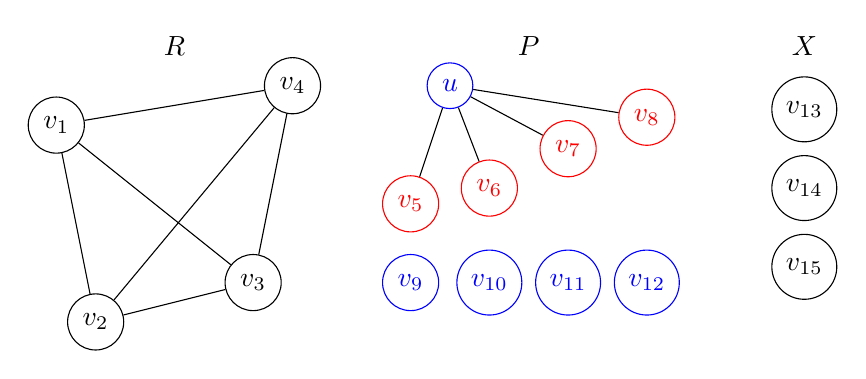
\begin{tikzpicture}
    \node (R) at (1.5, 2) {$R$};
    \node[draw, circle] (1) at (0, 1) {$v_1$};
    \node[draw, circle] (2) at (0.5, -1.5) {$v_2$};
    \node[draw, circle] (3) at (2.5, -1) {$v_3$};
    \node[draw, circle] (4) at (3, 1.5) {$v_4$};
    \draw (1) -- (2);
    \draw (1) -- (3);
    \draw (1) -- (4);
    \draw (2) -- (3);
    \draw (2) -- (4);
    \draw (3) -- (4);

    \node (P) at (6, 2) {$P$};
    \node[draw, circle, blue] (u) at (5, 1.5) {$u$}; \nodestar{u}{4}{1.6}{1.4}{1.2}{1}
    \node[draw, circle, red] (5) at (4.5, 0) {$v_5$}; \nodestar{5}{3.5}{0.4}{0.2}{0}{-0.2}
    \node[draw, circle, red] (6) at (5.5, 0.2) {$v_6$}; \nodestar{6}{4.5}{0.3}{0.1}{-0.1}{-0.3}
    \node[draw, circle, red] (7) at (6.5, 0.7) {$v_7$}; \nodestar{7}{5.5}{0.8}{0.6}{0.4}{0.2}
    \node[draw, circle, red] (8) at (7.5, 1.1) {$v_8$}; \nodestar{8}{6.5}{1.2}{1}{0.8}{0.6}
    \node[draw, circle, blue] (9) at (4.5, -1) {$v_9$}; \nodestar{9}{3.5}{-0.6}{-0.8}{-1}{-1.2}
    \node[draw, circle, blue] (10) at (5.5, -1) {$v_{10}$}; \nodestar{10}{4.5}{-0.6}{-0.8}{-1}{-1.2}
    \node[draw, circle, blue] (11) at (6.5, -1) {$v_{11}$}; \nodestar{11}{5.5}{-0.6}{-0.8}{-1}{-1.2}
    \node[draw, circle, blue] (12) at (7.5, -1) {$v_{12}$}; \nodestar{12}{6.5}{-0.6}{-0.8}{-1}{-1.2}

    \draw (u) -- (5);
    \draw (u) -- (6);
    \draw (u) -- (7);
    \draw (u) -- (8);

    \node (X) at (9.5, 2) {$X$};
    \node[draw, circle] (13) at (9.5, 1.2) {$v_{13}$}; \nodestar{13}{8.5}{1.4}{1.2}{1}{0.8}
    \node[draw, circle] (14) at (9.5, 0.2) {$v_{14}$}; \nodestar{14}{8.5}{0.4}{0.2}{0}{-0.2}
    \node[draw, circle] (15) at (9.5, -0.8) {$v_{15}$}; \nodestar{15}{8.5}{-0.3}{-0.5}{-0.7}{-0.9}
\end{tikzpicture}
    \caption{Rappresentazione dei tre insiemi $R$, $P$ e $X$ nel corso dell'algoritmo di Bron-Kerbosch con pivoting}
    \label{fig:bron_kerbosh_pivot_example}
\end{figure}

La figura~\ref{fig:bron_kerbosh_pivot_example} tenta di dare un'idea migliore degli insiemi R, P ed X nel corso
dell'esecuzione dell'algoritmo con strategia di pivoting.
Il nodo $u$ \'e scelto come pivot, e le chiamate ricorsive al livello corrente della ricorsione sono limitate ai nodi
in blu.
I segmenti uscenti da ogni nodo in P ed X rappresentano gli archi che li rendono adiacienti ad ogni nodo in R.

\begin{figure}[H]
    \centering
    \resizebox{!}{10cm}{
\begin{tikzpicture}[square/.style={regular polygon,regular polygon sides=4}]
	    %H0
	    \node (A) at (-9.15,1.4) [font=\scriptsize, text width=4em,square,draw]
	    	{\shortstack[l]{$Pivot=3$\\$ R=\emptyset$\\$P=\{1,2,3,4\}$\\$X=\emptyset$}};
	    %H1
	    \node (B) at (-11.5,-2.8) [font=\scriptsize, text width=4em,square,draw]
	    	{\shortstack[l]{$Pivot=1$\\$ R=\{3\}$\\$P=\{1,2,4\}$\\$X=\emptyset$}};

	    \node (C) at (-6.5,-2.8) [font=\scriptsize, text width=4em,square,draw]
	    	{\shortstack[l]{$Pivot=4$\\$ R=$\{5\}\\$P=\{4\}$\\$X=\emptyset$}};
            %H2
	    \node (D) at (-13,-6) [font=\scriptsize, text width=4em,square,draw]
	    	{\shortstack[l]{$Pivot=2$\\$ R=$\{3,1\}\\$P=\{2\}$\\$X=\emptyset$}};
	    \node (E) at (-10,-6) [font=\scriptsize, text width=4em,square,draw]
	    	{\shortstack[l]{$\color{blue}R=$\color{blue}\{3,4\}\\$P=\emptyset$\\$X=\emptyset$}};

	    \node (F) at (-6.5,-6) [font=\scriptsize, text width=4em,square,draw]
	    	{\shortstack[l]{$\color{blue}R=$\color{blue}\{5,4\}\\$P=\emptyset$\\$X=\emptyset$}};
	    %H4
	    \node (G) at (-13, -9) [font=\scriptsize, text width=4em,square,draw]
	    	{\shortstack[l]{$\color{blue}R=$\color{blue}\{3,1,2\}\\$P=\emptyset$\\$X=\emptyset$}};



	    %E0-1
	    \draw (A) to[out=270, in=90, looseness=0] (B);
	    \draw (A) to[out=270, in=90, looseness=0] (C);

	    %E1-2
	    \draw (B) to[out=270, in=90, looseness=0] (D);
	    \draw (B) to[out=270, in=90, looseness=0] (E);
	    \draw (C) to[out=270, in=90, looseness=0] (F);

	    %E2-3
	    \draw (D) to[out=270, in=90, looseness=0] (G);

	\begin{scope}[shift={(-16.5, 0.3)}]
		\node[circle, draw] (A) {1};
		\node[circle, draw] (B) [right of=A, node distance=2cm] {2};
		\node[circle, draw] (C) [above of=B, node distance=2cm] {3};
		\node[circle, draw] (D) [right  of=C, node distance=2cm] {4};
		\node[circle, draw] (E) [below of=D, node distance=2cm] {5};

		\draw(A) -- (B);
		\draw(B) -- (C);
		\draw(A) -- (C);
		\draw(C) -- (D);
		\draw(D) -- (E);
	\end{scope}
\end{tikzpicture}
}
    \caption{Esempio di albero di ricorsione dell'algoritmo di Bron-Kerbosch con pivoting}
    \label{fig:bron_kerbosh_pivot_tree_example}
\end{figure}

La figura ~\ref{fig:bron_kerbosh_pivot_tree_example} mostra l'albero di ricorsione derivante dall'applicazione
dell'algoritmo di Bron-Kerbosch con pivoting sullo stesso grafo orientato presente in figura
~\ref{fig:bron_kerbosh_tree_example}, rendendo evidente come la strategia di pivoting permetta di ridurre il numero
di chiamate ricorsive rispetto alla versione senza pivoting.

\paragraph{Complessit\'a}
Come dimostrato da Tomita ~\cite{TOMITA200628}, adottando una strategia di pivoting affinch\'e si scelga il nodo pivot
$w$ con il maggior numero di vicini in $P$, l'algoritmo di Bron-Kerbosch ha una complessit\'a temporale pari a
$O(3^{n/3})$, che \'e una complessit\'a ottimale, in quanto il numero massimo di cricche massimali che si possono
trovare in un grafo con $n$ nodi \'e dimostrato essere $3^{n/3}$.

\section{Enumerazione di circuiti semplici}\label{sec:enumerazione-di-cicli}

Come gi\`a spiegato nel capitolo introduttivo, un circuito semplice di un grafo diretto \'e un circuito
che non contiene nodi ripetuti, ad eccezione del nodo di partenza e di arrivo.
Dal momento in cui, per definizione, un circuito non pu\`o contenere archi ripetuti, parlare anche solo di cicli
semplici garantirebbe che esso non contenga neanche archi ripetuti.
Si potrebbe notare che, mentre componenti fortemente connesse e cricche sono concetti che possono essere
ricondotti ad un insieme non ordinato, i circuiti semplici comprendono in s\'e una sequenza di nodi in un determinato
ordine.
Per questo motivo diventa rilevante distinguere tra cicli e permutazioni cicliche, in quanto ogni ciclo
pu\`o essere rappresentato da un insieme di permutazioni cicliche.
Ad esempio, il ciclo $c_1 = \langle v_1, v_2, v_3, v_1 \rangle$ pu\`o essere rappresentato anche attraverso le
permutazioni cicliche $\langle v_2, v_3, v_1, v_2 \rangle$ e $\langle v_3, v_1, v_2, v_3 \rangle$, in quanto entrambe
rappresentano lo stesso anello di nodi percorsi nello stesso senso. \newline
\`E interessante notare che il ciclo $c_2 = \langle v_1, v_3, v_2, v_1 \rangle$, nonostante sia un ciclo semplice
composto degli stessi nodi di $c_1$, non pu\`o essere rappresentato da nessuna permutazione ciclica di $c_1$.
Per questo motivo due cicli si dicono distinti se non sono l'uno una permutazione ciclica dell'altro. \newline

In questa sezione tratteremo, quindi, un algoritmo per l'enumerazione di circuiti semplici in un grafo diretto, che
risolve il problema di individuare tutti i cicli semplici distinti presenti in un grafo diretto.


\subsection{Algoritmo di ricerca dei circuiti semplici di Johnson} \label{subsec:algoritmo-di-jhonson}
L'algoritmo per la ricerca dei circuiti semplici di Donald B. Johnson, proposto nel 1975~\cite{doi:10.1137/0204007},
provvede ad enumerare tutti i cicli in un grafo orientato eseguendo delle visite in profondit\`a. \newline

A partire da un ordinamento arbitrario dei nodi, l'algoritmo esegue la procedura di visita ricorsiva CIRCUIT partendo
da ciascuno di essi, individuando di volta in volta tutti e soli i circuiti semplici contenenti il nodo di partenza $s$.
Nel corso di ogni visita viene mantenuto uno stack $S$, su cui si effettua una operazione di $PUSH(S, v)$ non
appena $v$ viene visitato invocando la procedura CIRCUIT su $v$, e una operazione di $POP(S)$ non appena la visita
sul nodo termina.
Lo stack, quindi, rappresenta in ogni momento il prefisso di un potenziale circuito semplice che inizia e finisce in $s$.
Quando la visita a partire da un certo nodo $s$ si conclude, si considera il nuovo grafo ottenuto come grafo indotto
dal grafo precedente sui nodi rimanenti, ovvero il grafo della precedente iterazione privato del nodo $s$ e di tutti
gli archi incidenti su di esso.
Questo permette di evitare l'individuazione di tutti i circuiti equivalenti che sono permutazioni cicliche degli stessi
nodi. \newline

Tuttavia, quelle elencate non sono le sole caratteristiche che hanno determinato il successo dell'algoritmo.
Sebbene condivida con loro aspetti comuni, l'algoritmo risulta essere pi\`u efficente di altri algoritmi
proposti per lo stesso problema, come quello di Tiernan~\cite{10.1145/362814.362819} e
Weinblatt~\cite{10.1145/321679.321684}, in quanto utilizza un criterio di blocco
dei nodi che permette di evitare visite successive in aree del grafo che non conducono al nodo origine $s$.
Ogni nodo \`e bloccato nel corso di una visita, e viene sbloccato all'uscita solamente se esso conduce ad almeno
un cammino verso il nodo origine $s$ (che non si interseca con lo stack dei nodi correntemente visitati, mantenendo
la semplicit\`a del ciclo).
Ogni nodo $v$ custodisce una lista $v.B$ di nodi che, informalmente, pu\`o considerarsi come l'insieme di nodi
che sono stati bloccati a causa del blocco del nodo $v$ nel corso di una visita.
Per cui, quando un nodo viene sbloccato, la procedura UNBLOCK($v$) provvede a sbloccare non solo il nodo stesso $v$,
ma ricorsivamente anche tutti i nodi eventualmente presenti in $v.B$.

\begin{algorithm}[H] \floatname{algorithm}{Algoritmo}
    \caption{JHONSON-ALGORITHM($G$)}\label{alg:jhonson-algorithm}
    \begin{algorithmic}[1]
        \State Sia $S$ una pila di nodi vuota
        \State $i \coloneqq 1$
        \While {$i < n$}
            \State $K \coloneqq$ componente fortemente connessa contenente il vertice $v_i$
            nel sottografo indotto $G[\{v_i, v_{i+1}, \ldots, v_n\}]$
            \If {$K.E \neq \emptyset$}
                \State $s \coloneqq $ $v_i$
                \For {$u \in K.V$}
                    \State $u.blocked \coloneqq false$
                    \State $u.B \coloneqq \emptyset$
                \EndFor
                \State CIRCUIT($s, s, K, S$)
                \State $i \coloneqq i + 1$
            \Else
                \State $i \coloneqq n$
            \EndIf
        \EndWhile
    \end{algorithmic}
\end{algorithm}

\newpage

I parametri passati alla procedura ricorsiva CIRCUIT includono
\begin{itemize}
    \item il nodo da visitare $v$
    \item il nodo origine del circuito $s$
    \item il grafo indotto attuale $K$ su cui avviene la ricerca
    \item lo stack dei nodi attualmente in corso di visita $S$
\end{itemize}

\begin{algorithm}[h!] \floatname{algorithm}{Algoritmo}
    \caption{CIRCUIT($v, s, K, S$)}\label{alg:circuit}
    \begin{algorithmic}[1]
        \State $f \coloneqq false$
        \State $PUSH(S, v)$
        \State $v.blocked \coloneqq true$
        \For {$w \in K.adj[s]$}
            \If {$w == s$}
                \State Fornisci in output $S$ seguito da $s$ come un circuito semplice
                \State $f \coloneqq true$
            \ElsIf {$\lnot w.blocked$}
            \If {CIRCUIT($w$)} \State $f \coloneqq true$ \EndIf
            \EndIf
        \EndFor
        \If {$f$} UNBLOCK($v$)
        \Else
            \For {$w \in K.adj[v]$}
                \State $w.B \coloneqq w.B \cup \{v\}$
            \EndFor
        \EndIf
        \State $POP(S)$ \Comment{removes $v$ from stack}
        \State \textbf{return} $f$
    \end{algorithmic}
\end{algorithm}

%Al posto dell'output di un circuito:
%\State Let $C$ be a new simple circuit
%\For {$u \in S$}
%    \State $T[u] \coloneqq T[u] \cup \{C\}$
%\EndFor
\begin{algorithm}[H]
    \caption{UNBLOCK($v$)}\label{alg:unblock}
    \begin{algorithmic}[1]
        \State $v.blocked \coloneqq false$
        \For {$w \in v.B$}
            \State $v.B \coloneqq v.B \setminus \{w\}$
            \If {$w.blocked$} UNBLOCK($w$) \EndIf
        \EndFor
    \end{algorithmic}
\end{algorithm}

In Figura \label{fig:circuit-example} \`e fornita una rappresentazione delle fasi rilevanti dell'applicazione della
procedura CIRCUIT al nodo 1. I nodi in grigio rappresentano nodi bloccati.
La figura (a) mostra l'inzio della procedura, in cui il nodo 1 viene aggiunto allo tack $S$.
La figura (b) rappresenta il momento dell'individuazione del circuito $\langle 1, 3, 4, 1 \rangle$, derivante dalla valutazione
dell'arco $(4, 1)$.
La figura (c) rappresenta gli effetti della procedura CIRCUIT(5), derivante dalla valutazione dell'arco $(4, 5)$.
La figura (d) rappresenta gli effetti della procedura CIRCUIT(7), derivante dalla valutazione dell'arco $(4, 7)$.
In entrambe le figure (c) e (d) i nodi visitati vengono aggiunti e rimossi dallo stack, ma rimangono bloccati,
in quanto non conducono ad un circuito elementare, e per questo vengono aggiornate le liste $B$ dei relativi
nodi adiacenti.
Le figure (e) e (f) raffigurano le procedure ricorsive di UNBLOCK derivanti dallo sblocco del nodo 4.

\begin{figure}[!h] \centering
    \resizebox{!}{5.3cm}{
        \begin{tikzpicture}
            \node[mynode, fill={rgb:black,1;white,2}, label={[align=center]above:{\small $B = \emptyset$}}](n1) at (0,-1){1};
            \node[mynode, fill=white, label={[align=center]above:{\small $B = \emptyset$}}](n2) at (0,1.5){2};
            \node[mynode, fill=white, label={[align=left]right:{\small $B = \emptyset$}}](n3) at (4,-3){3};
            \node[mynode, fill=white, label={[align=left]right:{\small $B = \emptyset$}}](n4) at (4,0){4};
            \node[mynode, fill=white, label={[align=left]right:{\small $B = \emptyset$}}](n5) at (4,3){5};
            \node[mynode, fill=white, label={[align=center]below:{\small $B = \emptyset$}}](n6) at (8,-1.5){6};
            \node[mynode, fill=white, label={[align=center]above:{\small $B = \emptyset$}}](n7) at (8,1.5){7};

            \draw[myarrow](n1) -- (n3);
            \draw[myarrow](n2) -- (n4);
            \draw[myarrow](n3) -- (n4);
            \draw[myarrow](n3) -- (n6);
            \draw[myarrow](n4) -- (n1);
            \draw[myarrow](n4) -- (n5);
            \draw[myarrow](n4) -- (n7);
            \draw[myarrow](n5) -- (n2);
            \draw[myarrow](n6) -- (n4);
            \draw[myarrow](n7) -- (n5);
            \draw[myarrow](n7) -- (n6);

            \node[align=left, xshift=0cm, yshift=3cm] (label2) {$S = \langle 1 \rangle$};
            \node[below=10mm] at (4, -3.1) {\textbf{(a)}};
        \end{tikzpicture}

        \begin{tikzpicture}

            \node[mynode, fill={rgb:black,1;white,2}, label={[align=center]above:{\tiny $B = \emptyset$}}](n1) at (0,-1){1};
            \node[mynode, fill=white, label={[align=center]above:{\tiny $B = \emptyset$}}](n2) at (0,1.5){2};
            \node[mynode, fill={rgb:black,1;white,2}, label={[align=left]right:{\tiny $B = \emptyset$}}](n3) at (4,-3){3};
            \node[mynode, fill={rgb:black,1;white,2}, label={[align=left]right:{\tiny $B = \emptyset$}}](n4) at (4,0){4};
            \node[mynode, fill=white, label={[align=left]right:{\tiny $B = \emptyset$}}](n5) at (4,3){5};
            \node[mynode, fill=white, label={[align=center]below:{\tiny $B = \emptyset$}}](n6) at (8,-1.5){6};
            \node[mynode, fill=white, label={[align=center]above:{\tiny $B = \emptyset$}}](n7) at (8,1.5){7};

            \draw[myarrow, color=red](n1) -- (n3);
            \draw[myarrow](n2) -- (n4);
            \draw[myarrow, color=red](n3) -- (n4);
            \draw[myarrow](n3) -- (n6);
            \draw[myarrow, color=red](n4) -- (n1);
            \draw[myarrow](n4) -- (n5);
            \draw[myarrow](n4) -- (n7);
            \draw[myarrow](n5) -- (n2);
            \draw[myarrow](n6) -- (n4);
            \draw[myarrow](n7) -- (n5);
            \draw[myarrow](n7) -- (n6);

            \node[align=left, xshift=0cm, yshift=3cm] (label2) {$S = \langle 1, 3, 4 \rangle$};
            \node[below=10mm] at (4, -3.2) {\textbf{(b)}};
        \end{tikzpicture}
    }
\end{figure}

\begin{figure}[!h] \centering
    \resizebox{!}{5.3cm}{
        \begin{tikzpicture}
            \node[mynode, fill={rgb:black,1;white,2}, label={[align=center]above:{\tiny $B = \emptyset$}}](n1) at (0,-1){1};
            \node[mynode, fill={rgb:black,1;white,2}, label={[align=center]above:{\tiny $B = \{5\}$}}](n2) at (0,1.5){2};
            \node[mynode, fill={rgb:black,1;white,2}, label={[align=left]right:{\tiny $B = \emptyset$}}](n3) at (4,-3){3};
            \node[mynode, fill={rgb:black,1;white,2}, label={[align=left]right:{\tiny $B = \{2\}$}}](n4) at (4,0){4};
            \node[mynode, fill={rgb:black,1;white,2}, label={[align=left]right:{\tiny $B = \emptyset$}}](n5) at (4,3){5};
            \node[mynode, fill=white, label={[align=center]below:{\tiny $B = \emptyset$}}](n6) at (8,-1.5){6};
            \node[mynode, fill=white, label={[align=center]above:{\tiny $B = \emptyset$}}](n7) at (8,1.5){7};

            \draw[myarrow, color=red](n1) -- (n3);
            \draw[myarrow, color=red](n2) -- (n4);
            \draw[myarrow, color=red](n3) -- (n4);
            \draw[myarrow](n3) -- (n6);
            \draw[myarrow](n4) -- (n1);
            \draw[myarrow, color=red](n4) -- (n5);
            \draw[myarrow](n4) -- (n7);
            \draw[myarrow, color=red](n5) -- (n2);
            \draw[myarrow](n6) -- (n4);
            \draw[myarrow](n7) -- (n5);
            \draw[myarrow](n7) -- (n6);

            \node[align=left, xshift=0cm, yshift=3cm] (label2) {$S = \langle 1, 3, 4 {\color{red}, 5, 2} \rangle$};
            \node[below=10mm] at (4, -3.2) {\textbf{(c)}};
        \end{tikzpicture}

        \begin{tikzpicture}
            \node[mynode, fill={rgb:black,1;white,2}, label={[align=center]above:{\tiny $B = \emptyset$}}](n1) at (0,-1){1};
            \node[mynode, fill={rgb:black,1;white,2}, label={[align=center]above:{\tiny $B = \{5\}$}}](n2) at (0,1.5){2};
            \node[mynode, fill={rgb:black,1;white,2}, label={[align=left]right:{\tiny $B = \emptyset$}}](n3) at (4,-3){3};
            \node[mynode, fill={rgb:black,1;white,2}, label={[align=left]right:{\tiny $B = \{2, 6\}$}}](n4) at (4,0){4};
            \node[mynode, fill={rgb:black,1;white,2}, label={[align=left]right:{\tiny $B = \{7\}$}}](n5) at (4,3){5};
            \node[mynode, fill={rgb:black,1;white,2}, label={[align=center]below:{\tiny $B = \{7\}$}}](n6) at (8,-1.5){6};
            \node[mynode, fill={rgb:black,1;white,2}, label={[align=center]above:{\tiny $B = \emptyset$}}](n7) at (8,1.5){7};

            \draw[myarrow, color=red](n1) -- (n3);
            \draw[myarrow](n2) -- (n4);
            \draw[myarrow, color=red](n3) -- (n4);
            \draw[myarrow](n3) -- (n6);
            \draw[myarrow](n4) -- (n1);
            \draw[myarrow](n4) -- (n5);
            \draw[myarrow, color=red](n4) -- (n7);
            \draw[myarrow](n5) -- (n2);
            \draw[myarrow, color=red](n6) -- (n4);
            \draw[myarrow, color=red](n7) -- (n5);
            \draw[myarrow, color=red](n7) -- (n6);

            \node[align=left, xshift=0cm, yshift=3cm] (label2) {$S = \langle 1, 3, 4 {\color{red}, 7, 6} \rangle$};
            \node[below=10mm] at (4, -3.2) {\textbf{(d)}};
        \end{tikzpicture}
    }
\end{figure}

\begin{figure}[!h] \centering
\resizebox{!}{5.3cm}{
    \begin{tikzpicture}
        \node[mynode, fill={rgb:black,1;white,2}, label={[align=center]above:{\tiny $B = \emptyset$}}](n1) at (0,-1){1};
        \node[mynode, fill=white, label={[align=center]above:{\tiny $B = \{5\}$}}](n2) at (0,1.5){2};
        \node[mynode, fill={rgb:black,1;white,2}, label={[align=left]right:{\tiny $B = \emptyset$}}](n3) at (4,-3){3};
        \node[mynode, fill=white, label={[align=left]right:{\tiny $B = \emptyset$}}](n4) at (4,0){4};
        \node[mynode, fill={rgb:black,1;white,2}, label={[align=left]right:{\tiny $B = \{7\}$}}](n5) at (4,3){5};
        \node[mynode, fill=white, label={[align=center]below:{\tiny $B = \{7\}$}}](n6) at (8,-1.5){6};
        \node[mynode, fill={rgb:black,1;white,2}, label={[align=center]above:{\tiny $B = \emptyset$}}](n7) at (8,1.5){7};

        \draw[myarrow, color=red](n1) -- (n3);
        \draw[myarrow](n2) -- (n4);
        \draw[myarrow, color=red](n3) -- (n4);
        \draw[myarrow](n3) -- (n6);
        \draw[myarrow](n4) -- (n1);
        \draw[myarrow](n4) -- (n5);
        \draw[myarrow](n4) -- (n7);
        \draw[myarrow](n5) -- (n2);
        \draw[myarrow](n6) -- (n4);
        \draw[myarrow](n7) -- (n5);
        \draw[myarrow](n7) -- (n6);

        \node[align=left, xshift=0cm, yshift=3cm] (label2) {$S = \langle 1, 3, 4 \rangle$};
        \node[below=10mm] at (4, -3.2) {\textbf{(e)}};
    \end{tikzpicture}

    \begin{tikzpicture}
        \node[mynode, fill={rgb:black,1;white,2}, label={[align=center]above:{\tiny $B = \emptyset$}}](n1) at (0,-1){1};
        \node[mynode, fill=white, label={[align=center]above:{\tiny $B = \emptyset$}}](n2) at (0,1.5){2};
        \node[mynode, fill={rgb:black,1;white,2}, label={[align=left]right:{\tiny $B = \emptyset$}}](n3) at (4,-3){3};
        \node[mynode, fill=white, label={[align=left]right:{\tiny $B = \emptyset$}}](n4) at (4,0){4};
        \node[mynode, fill=white, label={[align=left]right:{\tiny $B = \emptyset$}}](n5) at (4,3){5};
        \node[mynode, fill=white, label={[align=center]below:{\tiny $B = \emptyset$}}](n6) at (8,-1.5){6};
        \node[mynode, fill=white, label={[align=center]above:{\tiny $B = \emptyset$}}](n7) at (8,1.5){7};

        \draw[myarrow, color=red](n1) -- (n3);
        \draw[myarrow](n2) -- (n4);
        \draw[myarrow](n3) -- (n4);
        \draw[myarrow](n3) -- (n6);
        \draw[myarrow](n4) -- (n1);
        \draw[myarrow](n4) -- (n5);
        \draw[myarrow](n4) -- (n7);
        \draw[myarrow](n5) -- (n2);
        \draw[myarrow](n6) -- (n4);
        \draw[myarrow](n7) -- (n5);
        \draw[myarrow](n7) -- (n6);

        \node[align=left, xshift=0cm, yshift=3cm] (label2) {$S = \langle 1, 3, {\color{red}4} \rangle$};
        \node[below=10mm] at (4, -3.2) {\textbf{(f)}};
    \end{tikzpicture}
}
\caption{Fasi rilevanti dell'applicazione della procedura CIRCUIT}\label{fig:cicruit-example}
\end{figure}

\newpage

\paragraph{Complessit\`a}\label{subsec:complessit`a}
Come discusso nella trattazione originale \cite{doi:10.1137/0204007}, la complessit\`a dell'algoritmo di Johnson
\`e $O((n + m)(c + 1))$, dove $n$ \`e il numero di nodi, $m$ il numero di archi e $c$ il numero di circuiti semplici
presenti nel grafo.
Questo risultato \`e ottenuto considerando che tutti i nodi e gli archi del grafo possono essere visitati al pi\`u una
volta per ogni circuito elementare presente, ovvero che l'algoritmo impiega al pi\`u $O(n + m)$ tempo tra l'output di
un circuito e l'individuazione del successivo.
In particolare, ciascun nodo pu\`o essere bloccato al pi\`u una volta per ogni circuito, e non pu\`o passare pi\`u di
di $O(n + m)$ tempo tra il blocco di un nodo e il suo sblocco. \newline

Si noti tuttavia che, pur essendo l'algoritmo di Johnson pi\`u efficiente rispetto ad altri algoritmi proposti, la
complessit\`a computazionale nel caso peggiore (ovvero quello di un grafo completo) risulta essere maggiore dell'
esponenziale, dovuto al numero di circuiti semplici presenti, che in tal caso \`e pari a

\begin{equation*}
    c \quad = \quad \sum_{i = 1}^{n-1} \binom{n}{n-i+1} (n-1)!
\end{equation*}

\subsection{Algoritmo di ricerca dei circuiti semplici massimali} \label{sec:maximal-circuits}
L'algoritmo di Johnson pu\`o essere modificato per individuare i circuiti semplici massimali, ovvero i circuiti
semplici i cui nodi non sono inclusi nei nodi di altri circuiti semplici pi\`u grandi.\newline
Una tale modifica pu\`o essere ottenuta inserendo la procedura di controllo ADD-MAXIMAL-SUBSET all'interno della
procedura CIRCUIT a riga 6, al posto della normale aggiunta del sottoinsieme $S$ con ADD-SUBSET, in modo da verificare
che il circuito individuato sia massimale o meno rispetto ai nodi visitati.

Tale procedura sar\`a decritta nel dettaglio nel paragrafo successivo.


